Previously, we talked about \textbf{satisfaction}: since we have constraints, the solution must satisfy all of them simultaneously. Anyway,
sometimes we need to deal with \textbf{optimization}, that it's the same thing as before but there is an additional term, named \textbf{objective function}. \vspace{7pt}

In this case, the formal definition of a \textbf{Constraint Optimization Problem} is described also by $f$, the formalization of the optimization 
criterion as an objective function. Therefore, our original triple becomes $\langle \textbf{X,D,C,f} \rangle$, where:
\begin{itemize}
    \renewcommand{\labelitemi}{-}
    \item \textbf{X} set of decision variables.
    \item \textbf{D} set of domains of the decision variables.
    \item \textbf{C} set of constraints applied to the decision variables.
    \item \textbf{f} formalization of the optimization criterion. It can be a \textbf{minimization objective} (\textit{minimize f}) or a \textbf{maximization objective} (\textit{maximize $-f$}).
\end{itemize}
Let's take a look at the following problems, understanding what decision variables, domains and constraints are really.
\begin{example}[title = N-Queens]
    e.g. Place $n$ queens in an $n \times n$ board so that no two queens can attack each other. \vspace{3.5pt}
    \begin{center}
        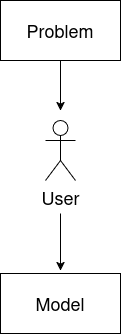
\includegraphics[width = 0.3\textwidth]{img/img1.png}
    \end{center} \vspace{3.5pt}
    There are many ways to model this problem, however we try to solve it using the obvious approach. Our goal is to place $n$ queens in a such way there is only 
    one of them for each row, column and diagonal. We begin by defining the decision variables and their domains. \vspace{7pt}

    \textbf{Decision variables and domains}.
    \begin{itemize}
        \renewcommand{\labelitemi}{-}
        \item Since each row must contain exactly only one queen, we define $n$ decision variables $[X_1, X_2, \dots, X_n]$; mapping one variable at each row we can satisfy the \textit{no row attack} condition.
        \item The domain values $\{1, \dots, n\}$ represent the available columns. An assignment $X_i = j$ indicates that queen in row $i$ is positionated in column $j$.
    \end{itemize} \vspace{7pt}

    To ensure no two queens attack each other, we must address three types of constraints:
    \begin{enumerate}
        \item \textit{Row attacks}.
        \item \textit{Column attacks}.
        \item \textit{Diagonal attacks}.
    \end{enumerate}
    Our modelling choice about decision variables allows us to satisfy the row constraint by design. Because each $X_i$ represents a distinct row, we only need 
    to explicitly define constraints for the remaining two. \vspace{7pt}

    \textbf{Constraints}.
    \begin{itemize}
        \renewcommand{\labelitemi}{-}
        \item $\textbf{alldifferent}([X_1, X_2, \dots, X_n])$.
        \item $\text{for all } i < j$ $|X_i - X_j| \neq |i-j|$.
    \end{itemize}
    These constraints prevent column and diagonal attacks, respectively. Specifically, the second constraint ensures that no two queens occupy the same diagonal,
    which occurs when the distance between their colums is equal to the distance between their rows.
\end{example}
\begin{example}[title = Sudoku]
    e.g. Sudoku. \vspace{3.5pt}
    \begin{center}
        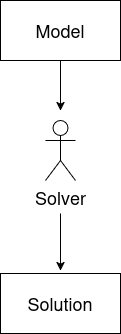
\includegraphics[width = 0.3\textwidth]{img/img2.png}
    \end{center} \vspace{3.5pt}
    Solving the famous sudoku problem, we can do something similar to the previous example. Even in this problem, we get some decision making processes subject 
    to constraints. As before, we begin by defining the decision variables. \vspace{7pt}

    \textbf{Decision variables}. \\
    We start modelling the decision variables, which are in this case the \textbf{empty cells}: for every cell we have to give a decision. Anyway,
    focusing only on the empty cells we cannot model properly the given problem; also, the already assigned cells can somehow influence our decisions. \vspace{7pt}

    \textbf{So, what do we do?} \\
    Simply, in our model these variables will be assigned to the current values shown in the image. \vspace{7pt}

    \textbf{Domains}. \\ 
    The domain values are any value in the set $\{1, \dots, 9\}$. \vspace{7pt}

    Summing up, we can create $9 \times 9$ different decision variables, where each of them has a domain \{1, \dots, 9\}; except for those variables that are 
    already associated to a value. \vspace{3.5pt}
    \begin{center}
        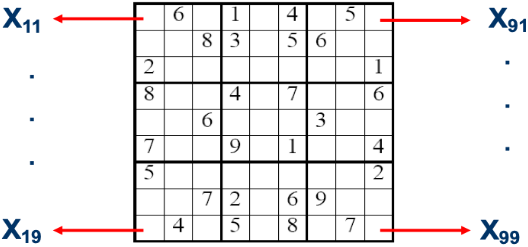
\includegraphics[width = 0.6\textwidth]{img/img3.png}
    \end{center} \vspace{7pt}

    \textbf{Constraints}. 
    \begin{itemize}
        \renewcommand{\labelitemi}{-}
        \item $\textbf{alldifferent}([X_{11}, X_{21}, X_{31}, \dots, X_{91}])$.
        \item $\textbf{alldifferent}([X_{11}, X_{12}, X_{13}, \dots, X_{19}])$.
        \item $\textbf{alldifferent}([X_{11}, X_{21}, X_{31}, X_{12}, X_{22}, X_{32}, X_{13}, X_{23}, X_{33}])$.
        \item Initial assignments, already described in the image (\textit{for instance, $X_{21} = 6$}).
    \end{itemize}
    The first three constraints ensure different values for any row, column and box of the sudoku table.
\end{example}
\begin{example}[title = Map colouring]
    e.g. Optimal map colouring. \vspace{3.5pt}
    \begin{center}
        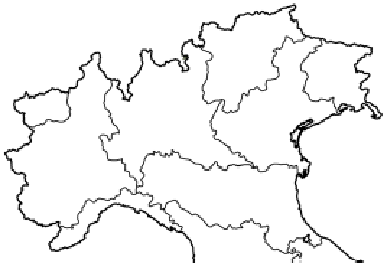
\includegraphics[width = 0.3\textwidth]{img/img4.png}
    \end{center} \vspace{3.5pt}
    Our goal is to colour regions such that neighboring regions are assigned different colors, using the minimum number of colors. \vspace{7pt}

    \textbf{Decision variables and domains}. \\
    Every decision variable would be a region and any single domain value represents a different color. More formally, $X_i$ with $i \in \{1, \dots, n\}$ are 
    the decision variables, while $\{1, \dots, n\}$ it's the domain. \vspace{7pt} 

    Since we have $n$ regions, we could use $n$ different colors satisfying the map colouring problem. However, we want to find out the minimum number of colors
    that we can use. \vspace{7pt}

    \textbf{Constraints}. 
    \begin{itemize}
        \renewcommand{\labelitemi}{-}
        \item $X_i \neq X_j \text{ for each neighboring region } i \text{ and } j$.
    \end{itemize}
    We specify inside the constraint the necessary condition for stating when a region is a neighbor of an other one, since not all the regions 
    are consecutive between each other. \vspace{7pt}

    \textbf{Objective variable}.
    \begin{itemize}
        \renewcommand{\labelitemi}{-}
        \item $f = max(X_i)$ \\ 
        where: 
        \begin{itemize}
            \item $X_i \rightarrow$ number of colors used by the map colouring
            \item $max(\dots) \rightarrow$ function used to detect how many colors were used 
        \end{itemize}
    \end{itemize}

    \textbf{Objective}. \\
    In order to obtain the minimum number of colors for the map colouring problem we have to minimize the objective function $f$.
\end{example}